\documentclass{exam}
\providecommand{\abs}[1]{\lvert#1\rvert}
\providecommand{\norm}[1]{\lVert#1\rVert}
\usepackage[utf8]{inputenc}
\usepackage[spanish, es-nolayout]{babel}		
\usepackage{amsmath}						
\usepackage{amsthm}							
\usepackage{amssymb}						
\usepackage{graphicx} 					
\usepackage{float}						
\usepackage{verbatim}					
\usepackage{url}								
\usepackage{subfig}				 
\usepackage{psfrag}			
\usepackage{multicol}
\usepackage{multirow}
\usepackage[bottom]{footmisc}
\usepackage{bigstrut}
\usepackage{color}
	\definecolor{ceruleanblue}{rgb}{0.16, 0.32, 0.75}
	\definecolor{coolblack}{rgb}{0.0, 0.18, 0.39}
	\definecolor{darkgreen}{rgb}{0.0, 0.2, 0.13}
\usepackage{multirow,hhline}
\usepackage{hyperref}
\hypersetup{
    colorlinks=true,
    linkcolor=black, % Color del enlace interno (por ejemplo, índice)
    urlcolor=black, % Color de los enlaces URL
    citecolor=black, % Color de las citas
}
\usepackage{tikz}



\usepackage{newtxmath}

\usepackage{physics}

\renewcommand{\thefootnote}{\fnsymbol{footnote}}


\pagestyle{headandfoot}					
\headrule 										

\firstpageheader{
\includegraphics[scale=0.2]{/Users/joaquin/Documents/GitHub/Ayudant-as-IO/Imágenes/Logo2.png}}{}{\scriptsize{Departamento de Economía} \\ \scriptsize{Facultad de Economía y Negocios}}
\runningheader{\scriptsize{
\includegraphics[scale=0.2]{/Users/joaquin/Documents/GitHub/Ayudant-as-IO/Imágenes/Logo2.png}}}{\scriptsize Microeconomía II \\ \scriptsize{Primavera 2024}} {\scriptsize{Departamento de Economía} \\ \scriptsize{Facultad de Economía y Negocios}}

\footrule
\footer{}{\scriptsize{P\'agina \thepage\ de \numpages}}{}
\parindent = 0pt
\renewcommand\partlabel{(\thepartno.)}
\renewcommand\thesubpart{\roman{subpart}}


\noprintanswers  
\renewcommand{\solutiontitle}{\noindent\textbf{Respuesta:}\par\noindent\sffamily}

\begin{document}
\begin{center}

\LARGE{\textbf{Microeconomía II}}

\medskip
\normalsize \textbf{Profesora:} Paola Bordón

\normalsize \textbf{Ayudantes:} Ayelén Sandoval, Diego Undurraga, Joaquín Martínez\footnote[2]{joamartine@fen.uchile.cl}


\medskip
\large{\textbf{Ayudantía 6}}

\end{center}

\tableofcontents

\renewcommand{\thefootnote}{\Roman{footnote}}

\section{Comentes}

\begin{itemize}
    \item[a)] Para el modelo de Cournot, la relación entre el índice de Herfindahl-Hirschman (IHH) y el índice de Lerner establece que una firma tiene alto poder de mercado si la elasticidad precio demanda es alta cuando la industria está concentrada. 
    \begin{solution}
        \textbf{Falso}. En el modelo de Cournot, al juntar el IHH \(\left( \sum s_i^2 \right)\) con el índice de Lerner \(\left( \frac{s_i}{\varepsilon_p} \right)\) se obtiene la siguiente relación:

\[
\bar{\lambda} = \sum_{i=1}^{N} s_i \lambda_i = \sum_{i=1}^{N} \frac{s_i^2}{\varepsilon_p} = \frac{IHH}{\varepsilon_p}
\]

Donde \(\bar{\lambda}\) y \(\lambda\) son los índice de Lerner y el índice de Lerner agregado respectivamente.

Lo que muestra que, pese a que una industria esté muy concentrada (tengo un alto IHH) una firma podría tener bajo poder de mercado si la demanda es muy elástica. En otras palabras, una firma tendría bajo poder cuando: 
\begin{itemize}
    \item[i)] Esté en un mercado muy atomizado y/o 
    \item[ii)] Enfrente una demanda muy elástica.
\end{itemize}
\end{solution}

\item [b)] Las fusiones deben ser prohibidas porque sólo empeoran a los consumidores. Comente.
\begin{solution}
    \textbf{Falso}. Si bien en algunos casos pueden generar concentraciones en mercados que pueden dañar a los consumidores, existen fusiones que pueden generar una ganancia de eficiencia tal que el precio baje, la cantidad aumente y los consumidores se vean beneficiados. Por lo tanto, las fusiones no siempre empeoran a los consumidores.
\end{solution}
\item[c)] Explique por qué razón las fusiones entre empresas con mayor participación de mercado a priori se consideran que tienen mayor posibilidad de incrementar los precios que aquellas entre firmas con menor participación de mercado. Emplee un modelo si es necesario.
\begin{solution}
    Si las firmas venden un producto homogéneo, es decir, sin diferenciación, aquellas de menor costo tendrán mayor participación de mercado. Por lo tanto, una fusión entre firmas de mayor participación de mercado implica que las de menores costos se fusionen y por lo tanto la principal firma competidora deja de competir, razón por la cual los precios tienden a subir más. Se puede emplear un modelo de Cournot o Bertrand para demostrar el resultado.
\end{solution}

\item[d)] En los modelos de entrada, siempre la mejor estrategia de la incumbente será bloquear la entrada.
\begin{solution}
    Falso. La firma tiene que analizar ambas decisiones en torno a la entrada de una nueva firma al mercado. Si el beneficio de acomodar la entrada de la firma es mayor al beneficio de bloquear la misma; la firma incumbente decidirá acomodar la entrada de la firma. En este sentido, es muy importante que la estrategia elegida sea creíble.
\end{solution}

\item[e)] La teoría de mercados desafiables nos diría que, ante pequeñas barreras de entradas, un mercado monopólico u oligopólico podría llegar a un equilibrio más similar al de competencia perfecta.

\begin{solution}
    Verdadero. La existencia de pocas barreras de entradas genera amenaza de competencia por parte de otras firmas, forzando a las incumbentes a comportarse de una manera más competitiva (i.e no hay poder de mercado independiente de la concentración).
\end{solution}


\end{itemize}

\section{Entrada con restricciones de capacidad}

Suponga que un mercado está caracterizado por la siguiente función de demanda lineal: \(p = 12 - Q\). La firma incumbente ($i = 1$) posee un costo marginal $c = 2$. Existe un potencial entrante ($i = 2$) que posee el mismo costo marginal que la incumbente, pero si entra, debe pagar un costo fijo de \(F = 2\). Suponga que tanto incumbente como entrante poseen una restricción de capacidad de \(k_i = 2\). \vspace{3mm}

En \(t = 1\), la firma entrante decide si ingresa o no al mercado, en caso que ingrese desembolsa \(F\). Si es que hay entrada en \(t = 2\) las firmas compiten Bertrand. Determine el precio, cantidades y beneficios de equilibrio si existiera entrada. ¿Existirá entrada en este mercado?

\begin{solution}
    Dado que hay restricciónes de capacidad la decisión de la entrante en $t = 2$ se reduce a ser demandante residual o recortador de precios. 

    \noindent
\begin{minipage}{0.45\textwidth}
    \textbf{Demandante residual:}\newline
    La cantidad residual será la cantidad demandada descontada por la cantidad que alcance a vender la incumbente. 
    \begin{align*}
        q_e &= 12 - \underbrace{k_1}_{k_1 = 2} - p_e \\
        q_e &= 10 - p_e 
    \end{align*}
    Por lo que se resuelve el problema de maximización con respecto a esta demanda. 
    \begin{align*}
        &\max_{p_e} \quad \pi_2 = (10-p_e)(p_e-2) \\
        \textbf{CPO:} \qquad &\pdv{\pi_e}{p_e} = 10-2p_e + 2 = 0 \rightarrow \boxed{p_e = 6}\\
        &q_e = 10 - 6 \to q_e = 4
    \end{align*}
    Dado que $q_e > k_2 = 2$ entonces $q_e$ pasa a ser 2. 
    \begin{align*}
        \boxed{q_e = 2, \quad p_e = 8}
    \end{align*}
    Los beneficios serán, 
    \begin{align*}
        \pi_e = (8-2)\cdot 2 \to \boxed{\pi_e = 12}
    \end{align*}
\end{minipage}%
\hfill%
\vrule width 1pt
\hfill%
\begin{minipage}{0.45\textwidth}
    \textbf{Recortar precios:}\newline
    Los beneficios de la empresa pasarán a describirse como,
    \begin{align*}
        \pi_p = (p_1-\epsilon -2) \cdot 2
    \end{align*}
    La condición para que entre recortando precios será,
    \begin{align*}
        \pi_p > \pi_e \\
        (p_1 - 2) \cdot 2 > 12 \to \boxed{p_1 > 8}
    \end{align*}
    Siempre que la firma incumbente ponga un precio mayor a $8$, la firma $2$ entra recortando precios. Por tanto, la función de reacción será:
    \[
        p_e =
        \begin{cases} 
        10 & \text{si } p_i > 10 \\
        p_i - \epsilon & \text{si } 8 < p_i < 10 \\
        8 & \text{si } p_i < 8
        \end{cases}
    \]
\end{minipage}
\vspace{3mm}
En \(t = 1\), la firma decide si entrar. Lo hará en cualquier escenario, ya que siempre recibe beneficios, y su costo de oportunidad es $0$.

\end{solution}



\section{Amenazas creíbles a la entrada}
Suponga una firma incumbente que se ve enfrentada a la entrada de una nueva firma. La demanda del mercado es \( Q = 20 - P \). Además, las firmas tienen costos marginales iguales a cero y tienen una capacidad fija. La firma entrante, en caso de entrar, empieza con una capacidad igual a 4. La incumbente no tiene costos de aumentar su capacidad. El precio estará dado por las capacidades ofrecidas, es decir, la cantidad será igual a la capacidad de cada firma y luego con eso se fija el precio.

Suponga que el juego funciona de la siguiente manera:

\textbf{t=1:} La firma entrante decide si entrar o no. En caso de no entrar, la firma entrante tiene un proyecto alternativo donde obtiene beneficios iguales a 16.

\vspace{3mm}

\noindent\textbf{t=2:} La firma incumbente decide si actuar agresivamente o no. En caso de actuar agresivamente, elige una capacidad que minimiza las utilidades de la firma entrante. En caso de no actuar agresivamente, maximiza sus utilidades.

\begin{itemize}
\item[a)] Plantee el juego y el árbol de decisión.
    \begin{solution}
        Para resolver el juego hay que calcular los pagos de las distintas alternativas.

        Primero, si la firma entrante no entra, recibirá un beneficio de 16 por su proyecto alternativo. La firma incumbente será un monopolio, y su beneficio será:
        \[
        \pi_i = 100
        \]

        Si la firma entrante ingresa y la incumbente actúa agresivamente, la incumbente elegirá una capacidad que minimice los beneficios de la entrante, es decir:
        \[
        \pi_E = P \cdot q_E = 0
        \]
        \[
        20 - q_I - 4 = 0
        \]
        Despejando, encontramos que la incumbente fija una capacidad de \( q_I = 16 \), y ambos, la firma incumbente y la entrante, tendrán beneficios iguales a 0.

        Si la firma entrante ingresa y la incumbente no actúa agresivamente, la incumbente maximiza sus beneficios considerando la capacidad de la entrante. El problema es:
        \[
        \max_{q_I} \quad \pi_I = P \cdot q_I
        \]
        \[
        \max_{q_I} \quad (20 - q_I - 4) \cdot q_I
        \]
        De esto se obtiene que \( q_I = 8 \), el precio será 8, los beneficios de la firma entrante serán \( \pi_E = 32 \), y los de la incumbente \( \pi_I = 64 \).\newline
        \begin{center}
            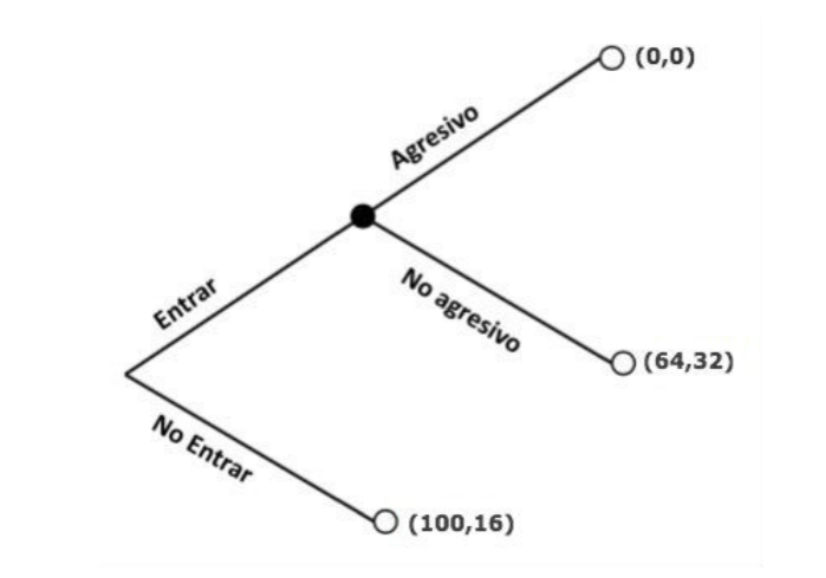
\includegraphics[width=0.5\linewidth]{/Users/joaquin/Documents/GitHub/Ayudant-as-IO/Primavera 2024/A6/arbol.png}
        \end{center}
        
    \end{solution}

    \item[b)] Encuentre el equilibrio y explique el resultado. ¿Qué rol juega el beneficio del proyecto alternativo de la firma entrante?
    \begin{solution}
        El equilibrio se resuelve por inducción hacia atrás. En la última etapa, la incumbente preferirá no actuar agresivamente, ya que obtiene mayores beneficios así. Sabiendo esto, la firma entrante preferirá ingresar al mercado, ya que la competencia no agresiva le reporta un beneficio mayor que su proyecto alternativo.

        A la incumbente le gustaría amenazar con actuar agresivamente para evitar la entrada y obtener un beneficio de \( \pi_I = 100 \), pero no puede hacer esta amenaza creíble. La razón es que, una vez que se produce la entrada, actuar agresivamente no es la mejor opción para la incumbente.

        El beneficio del proyecto alternativo de la firma entrante (\( 16 \)) representa el costo de oportunidad de la firma al decidir entrar o no. Si la firma entra y obtiene beneficios nulos, habría perdido el beneficio alternativo de 16.
    \end{solution}
    \item[c)] Suponga ahora que la firma incumbente puede elegir su capacidad antes de la entrada. ¿Cuál será la mejor opción de la incumbente en este caso?
    \begin{solution}
        En este caso, la incumbente puede fijar una capacidad para desincentivar la entrada de la competencia. Sin embargo, esta estrategia solo es conveniente si los beneficios son mayores que permitir la entrada, lo que anteriormente generaba una utilidad de \( \pi_I = 64 \).

        El nivel de capacidad que desincentiva la entrada es tal que los beneficios de la firma entrante sean menores que su proyecto alternativo:
        \[
        \pi_E = (20 - q_I - 4) \cdot 4 < 16
        \]
        \[
        q_I > 12
        \]
        Por lo tanto, la incumbente debe fijar una capacidad de al menos 13 unidades. Si lo hace, los beneficios serán los monopólicos menos los costos de inversión en capacidad:
        \[
        \pi_I = 100 - 3 \cdot 13 = 61
        \]
        Dado que estos beneficios son menores que \( \pi_I = 64 \), la mejor opción de la incumbente será permitir la entrada y escoger su capacidad posterior para maximizar sus beneficios.
    \end{solution}
\end{itemize}

\section{Propuesto: Fusiones Solemne Otoño 2024}

Suponga que Apple y Dell son los únicos competidores en el mercado de los notebooks. Suponga
que Apple y Dell venden productos diferenciados horizontalmente (Macbook y XPS) y compiten
en precios. Las funciones de demanda de Apple y Dell son:

\[
q_A = 2 - 2p_A + p_D,
\]
\[
q_D = 2 + p_A - 2p_D.
\]

Los costos marginales para ambas firmas son constantes e iguales a \( c_A = c_D = \frac{1}{2} \).

\begin{itemize}
    \item[a)] Encuentre los precios, cantidades y beneficios de cada firma en el equilibrio de Nash en precios. Grafique la funciones de mejor respuesta y el equilibrio.
    \begin{solution}
        Apple maximiza la siguiente función de beneficios:
        \[
        \max_{p_A} \quad \pi_A(p_A, p_D) = (p_A - c_A) q_A = (p_A - \frac{1}{2}) (2 - 2 p_A + p_D)
        \]
        Derivando con respecto al precio \(p_A\):
        \[
        \frac{\partial \pi_A(p_A)}{\partial p_A} = (2 - 2 p_A + p_D) - 2(p_A - \frac{1}{2}) = 3 - 4 p_A + p_D = 0
        \]
        Despejando la mejor respuesta de Apple:
        \[
        p_A(p_D) = \frac{3}{4} + \frac{1}{4} p_D
        \]

        En el equilibrio simétrico, \( p_A = p_D \). Entonces:
        \[
        3 - 4 p_A + p_A = 0
        \]
        \[
        3 - 3 p_A = 0 \quad \Rightarrow \quad p_A = p_D = 1
        \]
        Las cantidades serán:
        \[
        q_A = q_D = 1
        \]
        Los beneficios de cada firma serán:
        \[
        \pi_A = \pi_D = \frac{1}{2}
        \]
    \end{solution}

    \item[b)] Suponga que Apple y Dell deciden fusionarse y formar Dellapple que se comportará como un monopolista multiproducto (sin sinergias como consecuencia de la fusión). Encuentre los precios, cantidades y beneficios del monopolista multiproducto.
    \begin{solution}
        Dellapple maximiza la suma de beneficios de ambos productos:
        \[
        \max_{p_A, p_D} \quad \pi_A(p_A, p_D) + \pi_D(p_A, p_D) = (p_A - \frac{1}{2}) (2 - 2 p_A + p_D) + (p_D - \frac{1}{2}) (2 - 2 p_D + p_A)
        \]
        Derivamos la función de beneficios con respecto a \(p_A\):
        \[
        \frac{\partial (\pi_A + \pi_D)}{\partial p_A} = (2 - 2 p_A + p_D) - 2(p_A - \frac{1}{2}) + (p_D - \frac{1}{2}) = \frac{5}{2} - 4 p_A + 2 p_D = 0
        \]
        Usando la simetría \( p_A = p_D \):
        \[
        \frac{5}{2} - 4 p_A + 2 p_A = 0 \quad \Rightarrow \quad \frac{5}{2} - 2 p_A = 0 \quad \Rightarrow \quad p_A = p_D = \frac{5}{4}
        \]
        Las cantidades serán:
        \[
        q_A = q_D = \frac{3}{4}
        \]
        Los beneficios de Dellapple serán:
        \[
        \pi_A = \pi_D = \frac{9}{8}
        \]
    \end{solution}

    \item[c)] Explique por qué las firmas al actuar en forma independiente en (a) obtienen menos beneficios que un monopolista multiproducto.
    \begin{solution}
        Cuando las firmas toman decisiones de manera independiente, se encuentran en una situación similar al dilema del prisionero. Aunque existen precios más altos que maximizarían los beneficios conjuntos, cada firma tiene incentivos a reducir su precio unilateralmente para aumentar sus beneficios. Esto genera una externalidad negativa.

        Por el contrario, el monopolista multiproducto (Dellapple) tiene en cuenta tanto el efecto de los precios de Apple sobre la demanda de Dell como viceversa, lo que le permite fijar precios más altos y, en consecuencia, obtener mayores beneficios.
    \end{solution}

    \item[d)] ¿Los consumidores prefieren que las firmas compitan (como en (a)) o que exista un monopolista (como en (b))? ¿Su respuesta sería distinta si los bienes fuesen complementarios en lugar de sustitutos? Explique.
    \begin{solution}
        Los consumidores prefieren que las firmas compitan (como en el escenario de (a)) porque los precios son más bajos, lo que aumenta el excedente del consumidor. En este escenario, los productos son sustitutos, por lo que la competencia entre las firmas lleva a precios más bajos.

        Si los bienes fueran complementarios en lugar de sustitutos, los consumidores preferirían un monopolio (como en el escenario de (b)). En este caso, el monopolista tiene en cuenta la externalidad positiva que se genera entre los productos complementarios, lo que conduce a precios más bajos que en el escenario competitivo.
    \end{solution}
\end{itemize}

\end{document}